
\section{Σχεσιακό μοντέλο}

\subsection{Πεδία ορισμού}


\begin{tabular}{|p{6cm}|p{6cm}|}
\hline
  Πεδίο Ορισμού & Τύπος \\ \hline
  Ακέραιος & INT \\ \hline
  Όνομα & VARCHAR(40) \\ \hline
  Εκδηλώσεις & ENUMERATED\{Μουσική, Παράσταση, Ταινία, Σπορ,
               Εκδήλωση\} \\ \hline
  Δυαδικό & ENUMERATED\{Ναι, Όχι\} \\ \hline
  Κείμενο & VARCHAR(140) \\ \hline
  Διεύθυνση & VARCHAR(35) \\ \hline
  
… & … \\ \hline
\end{tabular}

\subsection{Σχέσεις}

(Προσδιορίστε τις σχέσεις του σχεσιακού μοντέλου.)

Παράδειγμα για τη FlightsDB:

Γνωρίσματα:

\begin{tabular}{|p{6cm}|p{6cm}|}
  \hline
  Όνομα Σχέσης & Airport \\ \hline
  \multicolumn{2}{|l|}{\textbf{Γνωρίσματα:}} \\ \hline
  Όνομα & Τύπος \\ \hline
  airport\_code & Κωδ\_Αεροδρομίου \\ \hline
  name & Απλό\_Αλφαριθμητικό \\ \hline
  city & Διεύθυνση \\ \hline
  country & Διεύθυνση \\ \hline
  \multicolumn{2}{|l|}{\textbf{Περιορισμοί Ακεραιότητας:}} \\ \hline
  Πρωτεύον Κλειδί & airport\_code \\ \hline
  Ξένα Κλειδιά & - (αναφέρετε κλειδί και σχ. σχέση, π.χ. air\_code ->
                 Airport) \\ \hline
\end{tabular}

\subsection{Σχεσιακό Σχήμα}

(Δείξτε το σχεσιακό σχήμα για τη βάση. Το σχήμα μπορείτε να το
κατασκευάσετε σε πρόγραμμα της επιλογής σας, ωστόσο θα πρέπει να
ακολουθεί το συμβολισμό του μαθήματος (δηλαδή οι σχέσεις ως κεφαλίδες
πινάκων, τα ξένα κλειδιά ως βέλη μιας κατεύθυνσης, κτλ.))

Παράδειγμα για τη FlightsDB (προσοχή το παράδειγμα δεν είναι πλήρως
αντίστοιχο με το διάγραμμα E/R που δόθηκε παραπάνω – για την εργασία
θα πρέπει να είναι πλήρως αντίστοιχα):

\begin{figure}[H]
  \centering
  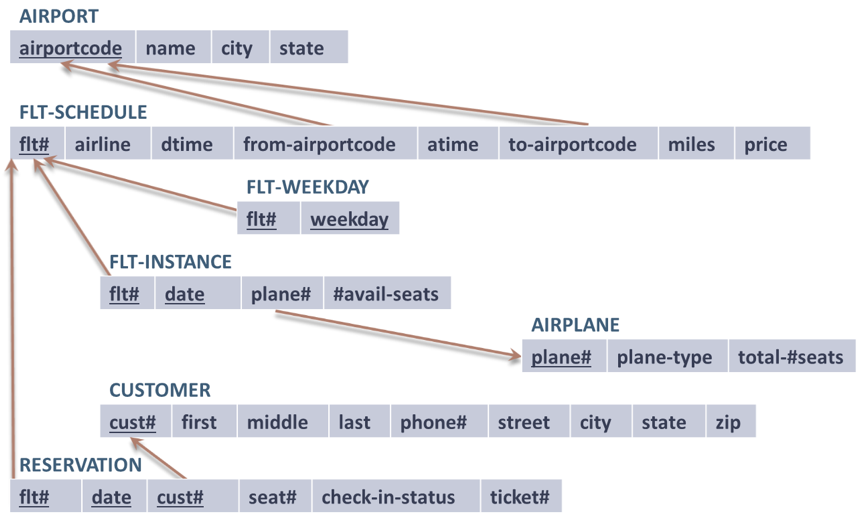
\includegraphics[width=.8\linewidth]{relations.png}
  \caption{Σχεσιακό μοντέλο}
\end{figure}

\subsection{Όψεις}
(Κατασκευάστε χρήσιμες όψεις για τη βάση. Κάθε όψη θα πρέπει να
οριστεί με σχεσιακή άλγεβρα)

Παράδειγμα για τη FlightsDB:

έστω η σχέση:

\begin{itemize}[noitemsep]
\item FLIGHT(flight\_id, airline, fromairport, toairport, price,
  plane\_id)
\item AIRPLANE(plane\_id, plane\_name) 
\end{itemize}

Μια όψη που περιέχει όλες τις αεροπορικές εταιρίες που υπάρχουν στο
σύστημα και τα ονόματα των αεροπλάνων που χρησιμοποιούν είναι η
παρακάτω:

ρAIRLINES(πairline, plane\_name(πairline, plane\_id(FLIGHT)
πplane\_id, plane\_name(AIRPLANE)))



%%% Local Variables:
%%% mode: latex
%%% TeX-master: "main"
%%% End:
